\chapter{Food 2}

\begin{itemize}
\tightlist
\item
  \textbf{NP 23,} Over-kept tonics
\item
  \textbf{Pc 31,} Public alms centre
\item
  \textbf{Pc 32,} Four bhikkhus specifically invited
\item
  \textbf{Pc 33,} Meal before invitation
\item
  \textbf{Pc 34,} More than three bowlfuls
\item
  \textbf{Pc 35,} More food after turning down what was offered
\item
  \textbf{Pc 36,} Tricking to break Pc 35
\item
  \textbf{Pc 41,} Handing food to members of other religions
\item
  \textbf{Pc 47,} Exceeding an invitation
\end{itemize}

\section{NP 23, Over-kept tonics}

{[}NP 23 Tonics{]}(./includes/mindmaps/np-23-tonics.png**

\begin{multicols}{2}

\textbf{Object:} any of the five tonics.

``There are these five tonics -- ghee, butter, oil, honey, and syrup --
that are generally regarded as tonics, serve the purpose of nourishment,
but are not considered as substantial food.''
(\href{https://suttacentral.net/pli-tv-kd6/en/brahmali}{Kd 6})

\textbf{Effort:} one keeps the tonic past the 7th dawnrise after
receiving it.

\textbf{Perception} is not a factor.

If one thinks the 7th dawn haven't passed, but it has, it is still NP.

If one thinks ``I receive \emph{this} salt as food for the morning, and
\emph{this} salt as medicine for later'', it may be a personal practice,
but not part of the rule. It doesn't affect the period of how long the
item may be used by oneself or any other bhikkhu.

\end{multicols}

\clearpage

\textbf{Origin:} Ven. Pilindavaccha receives an abundance of tonics, and
shares with his monks. They begin to ``fill up basins and waterpots and
setting these aside, they filled their water filters and bags and hung
these in the windows. The tonics were dripping all over and the
dwellings became infested with rats.''
(\href{https://suttacentral.net/pli-tv-bu-vb-np23/en/brahmali}{NP 23})

\textbf{Mixing:} The mixture takes on the shortest lifetime of the
ingredients. (Mv. VI.40.3.)

\begin{center}
\begin{tabular}{llllllll}
a. & 1d juice & rec. that morning & + & food & rec. that morning & \(\rightarrow\) & that morning\\
\hline
b. & 7d tonic & rec. that morning & + & food & rec. that morning & \(\rightarrow\) & that morning\\
\hline
c. & lifetime medicine & rec. that morning & + & food & rec. that morning & \(\rightarrow\) & that morning\\
\hline
d. & 7d tonic & rec. sometime & + & juice & rec. that day & \(\rightarrow\) & until dawn\\
\hline
e. & lifetime medicine & rec. sometime & + & juice & rec. that day & \(\rightarrow\) & until dawn\\
\hline
f. & lifetime medicine & rec. sometime & + & 7d tonic & rec. sometime & \(\rightarrow\) & 7 days\\
\end{tabular}
\end{center}

\subsection{7 days}

\emph{Sattāha paramaṃ}, ``up to seven days''. The Vinaya counts days
from dawn to dawn, hence one may use a 7 day tonic \emph{until the 7th
dawn}.

Confusion arises from ``7 days'' meaning either ``for 7 days''
(interval) or ``on the 7th day'' (ordinal).

\vspace*{\baselineskip}
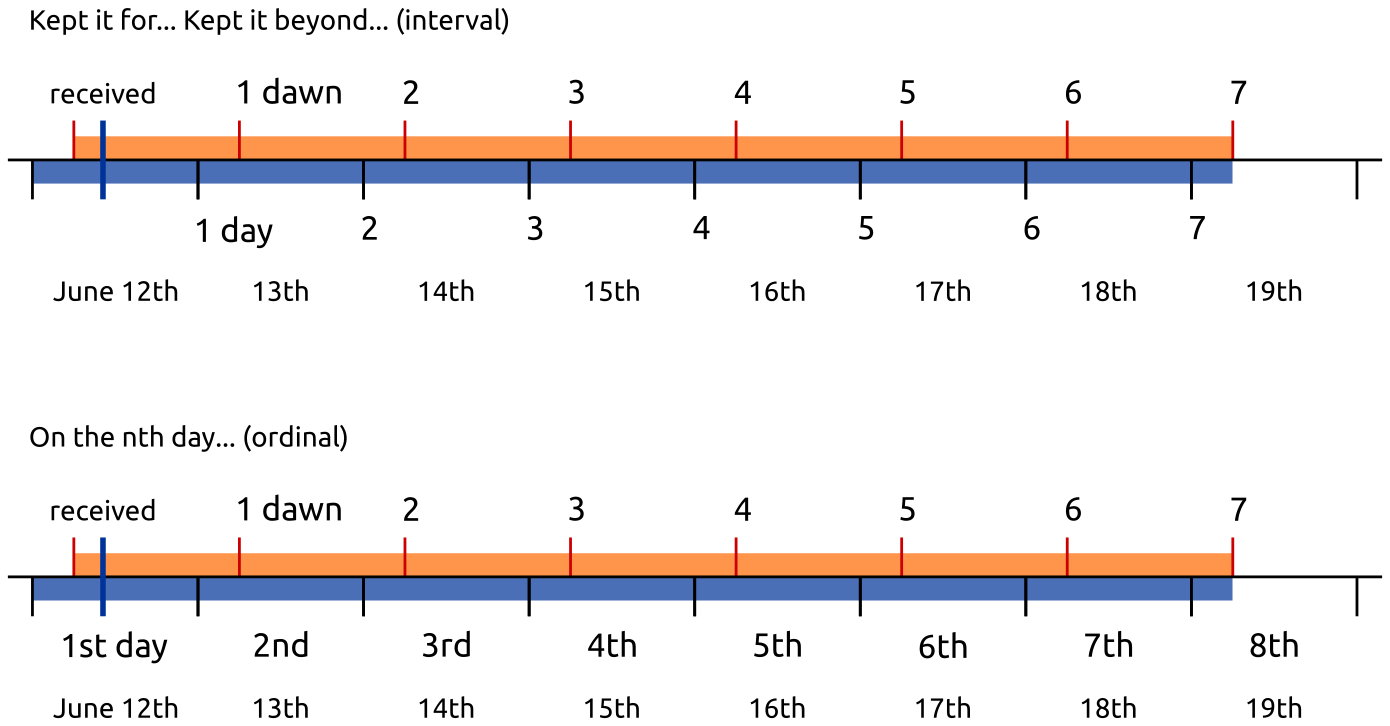
\includegraphics[width=\linewidth]{../../src/includes/figures/7-days.png}

\subsection{Breakfast tray}

After dawn, one receives a tray with bread, jams, honey, butter and
salt. At this point the lifetimes are:

\begin{itemize}
\tightlist
\item
  bread, jams: morning
\item
  honey, butter: 7 days
\item
  salt: lifetime
\end{itemize}

If the knife which one used carries bread morsels or jam into the honey
or the butter, these will be only allowable in the morning.

If one is careful to clean the knife and avoid mixing, one may use them
on the bread and keep the rest until their allowed lifetimes.

The next day, one receives a tray with only bread. One may \textbf{not}
mix the allowables from the previous day with the food received today.

Putting the salt, honey or butter (rec. yesterday) on the bread would be
Pc 38 (eating stored food).

\clearpage

\section{Pc 31, Public alms centre}

One may eat one meal at a public alms centre, not two or more days in a
row.

Origin: the group of six feel tired of almsround and keep going to the
same public kitchen.

Soup kitchens, homeless shelters, etc. Any place where all comers are
offered food free of charge.

\subsection{Non-offences}

\begin{itemize}
\tightlist
\item
  one is invited by the owners
\item
  being ill (not being able to leave)
\item
  the food is intended for bhikkhus
\item
  the centre limits the amount of food one may take (thus being able to
  censure a greedy person)
\end{itemize}

\section{Pc 32}

\section{Pc 33}

\section{Pc 34}

\section{Pc 35}

\section{Pc 36}

\section{Pc 41, Handing food to members of other religions}

One places oneself in the position of the followers of other religions.

It is not an offense to prepare food in a tray and placing it so that
they can help themselves.

\section{Pc 47, Exceeding an invitation}

When an invitation is made that one may ask for certain requisites, one
may use it until four months, unless it has been repeated, or is a
permanent invitation.

\subsection{Non-offenses}

\begin{multicols}{2}

\begin{itemize}
\tightlist
\item
  from relatives
\item
  for the sake of another
\item
  from one's own resources
\item
  being ill, if one shows consideration
\end{itemize}

\end{multicols}

``The time period for which we were invited has passed, but we have need
of medicine.''

